\documentclass[12pt]{article}

\include{preamble}

\newtoggle{professormode}
%\toggletrue{professormode} %STUDENTS: DELETE or COMMENT this line



\title{MATH 342W / 642 / RM742 Spring \the\year~HW \#1}

\author{Ye Htut Maung} %STUDENTS: write your name here

\iftoggle{professormode}{
\date{Due 11:59PM February 5~on github\\ \vspace{0.5cm} \small (this document last updated \currenttime~on \today)}
}

\renewcommand{\abstractname}{Instructions and Philosophy}

\begin{document}
\maketitle

\iftoggle{professormode}{
\begin{abstract}
The path to success in this class is to do many problems. Unlike other courses, exclusively doing reading(s) will not help. Coming to lecture is akin to watching workout videos; thinking about and solving problems on your own is the actual ``working out.''  Feel free to \qu{work out} with others; \textbf{I want you to work on this in groups.}

Reading is still \textit{required}. For this homework set, read the first chapter of \qu{Learning from Data} and the introduction and Chapter 1 of Silver's book. Of course, you should be googling and reading about all the concepts introduced in class online. This is your responsibility to supplement in-class with your own readings.

The problems below are color coded: \ingreen{green} problems are considered \textit{easy} and marked \qu{[easy]}; \inorange{yellow} problems are considered \textit{intermediate} and marked \qu{[harder]}, \inred{red} problems are considered \textit{difficult} and marked \qu{[difficult]} and \inpurple{purple} problems are extra credit. The \textit{easy} problems are intended to be ``giveaways'' if you went to class. Do as much as you can of the others; I expect you to at least attempt the \textit{difficult} problems. 

This homework is worth 100 points but the point distribution will not be determined until after the due date. See syllabus for the policy on late homework.

Up to 7 points are given as a bonus if the homework is typed using \LaTeX. Links to instaling \LaTeX~and program for compiling \LaTeX~is found on the syllabus. You are encouraged to use \url{overleaf.com}. If you are handing in homework this way, read the comments in the code; there are two lines to comment out and you should replace my name with yours and write your section. The easiest way to use overleaf is to copy the raw text from hwxx.tex and preamble.tex into two new overleaf tex files with the same name. If you are asked to make drawings, you can take a picture of your handwritten drawing and insert them as figures or leave space using the \qu{$\backslash$vspace} command and draw them in after printing or attach them stapled.

The document is available with spaces for you to write your answers. If not using \LaTeX, print this document and write in your answers. I do not accept homeworks which are \textit{not} on this printout. Keep this first page printed for your records.

\end{abstract}

\thispagestyle{empty}
\vspace{1cm}
NAME: \line(1,0){380}
\clearpage
}

\problem{These are questions about Silver's book, the introduction and chapter 1.}

\begin{enumerate}

\easysubproblem{What is the difference between \emph{predict} and \emph{forecast}? Are these two terms used interchangably today?}\spc{4}

Yes, these two terms are used interchangably today. A forecast is a planning under conditions of uncertainty and it came from English's Germanic roots. It has more like the way we now use the word foresight. A prediction is a predetermined future or a statement from a soothsayer.

\easysubproblem{What is John P. Ioannidis's findings and what are its implications?}\spc{5}

John's finding is that most of the positive findings documented in peer-reviewed journals and descriptions of successful predictions of medical hypotheses carried out in laboratory experiments were likely to fail when applied in the real world. It implies that many published scientific studies may be unreliable, leading to wrong treatments and wasted resources.

\easysubproblem{What are the human being's most powerful defense (according to Silver)? Answer using the language from class.}\spc{4}

The human being's most powerful defenses are our wits or our minds. We can identify patterns and find ways to measure those patterns. From those data, we generate models and predict the outcomes. If the outcome is true or close enough to real world, we make the model as a formula. For example, F = ma or E = m$c^2$.

\easysubproblem{Information is increasing at a rapid pace, but what is not increasing?}\spc{3}

The amount of useful information is not increasing. Most of it is just noise and the noise is increasing faster than the signal.

\hardsubproblem{Silver admits that we will always be subjectively biased when making predictions. However, he believes there is an objective truth. In class, how did we describe the objective truth? Answer using notation from class i.e. $t,f, g, h^*, \delta, \epsilon, t, z_1, \ldots, z_t, \delta, \mathbb{D}$, $\mathcal{H}, \mathcal{A}, \mathcal{X}, \mathcal{Y}, X, y, n, p$, $x_{\cdot 1}, \ldots, x_{\cdot p}, x_{1 \cdot}, \ldots, x_{n \cdot}$, etc.}\spc{3}

In class, we describe the objective truth as $y = t(z_1, z_2, \ldots, z_t)$ where $y$ is the outcome, $t$ is the exact functional relationship that can generate objective truth based on $z$ which are the true causes for $y$. However, since it is impossible to get exact/perfect $t$ and $z$, we use $f$ and $x$ to approximate $t$ and $z$. Moreover, we also need to consider $\delta$ for errors.


\easysubproblem{In a nutshell, what is Karl Popper's (a famous philosopher of science) definition of \emph{science}?}\spc{4}

In a nutshell, Karl Popper's definition of science is that a hypothesis was not scientific unless it can be proved wrong which means it is needed to test prediction with the real world data.

\intermediatesubproblem{Why did the ratings agencies say the probability of a CDO defaulting was 0.12\% instead of the 28\% that actually occured? Answer using concepts from class.}\spc{4}

The ratings agencies said the probability of a CDO defaulting was 0.12\% instead of 28\% that actually occurred because the default rates claimed by S\&P were not derived from historical data which is from $\mathbb{D}$. The securities were new and highly novel. Moreover, they were assumptions based on a faulty statistical model, which means that their function $f$ is probably bad and the error $\delta$ is huge.

\easysubproblem{What is the difference between \emph{risk} and \emph{uncertainty} according to Silver's definitions?}\spc{4}

Risk s something that you can put a price on which means you know the probability of winning or lose like a poker game. Uncertainty is risk that is hard to measure which means you don't know what will happen or what could happen.

\hardsubproblem{How does Silver define \emph{out of sample}? Answer using notation from class i.e. $t,f, g, h^*, \delta, \epsilon, z_1, \ldots, z_t, \delta, \mathbb{D}, \mathcal{H}, \mathcal{A}, \mathcal{X}, \mathcal{Y}, X, y, n, p, x_{\cdot 1}, \ldots, x_{\cdot p}, x_{1 \cdot}, \ldots, x_{n \cdot}$, etc. WARNING: Silver defines \emph{out of sample} completely differently than the literature, than practitioners in industry and how we will define it in class in a month or so. We will explore what he is talking about in class in the future and we will term this concept differently, using the more widely accepted terminology. So please forget the phrase \emph{out of sample} for now as we will introduce it later in class as something else. There will be other such terms in his book and I will provide this disclaimer at these appropriate times.}\spc{7}

Silver defines $out of sample$ by not having historical data of certain features that should account for the model. For example, he gives an example of not having the data of the past drinking experience of the diver could lead to forecast inaccurate accident risk. Using the notation form the class, when we collect the data for $x_1, x_2, x_3$, we only collect people from city which has high salary, low crime rate and good credit scores and test the model, the model could be accurate or good enough to approximate if a person could pay the loan back. However, if a person from a countryside  which has low salary, high crime rate and good credit scores lands a loan, the model cannot act accurately as it does not have the data from countryside which we can say it is $out of sample$.

\intermediatesubproblem{Look up \emph{bias} and \emph{variance} online or in a statistics textbook. Connect these concepts to Silver's terms \emph{accuracy} and \emph{precision}. This is another example of Silver using non-standard terminology.}\spc{9}

Bias is anything that leads to a systematic difference between the true parameters of a population and the statistics used to estimate those parameters. In other words, bias refers to a flaw in the experiment design or data collection process that generates results that do not accurately represent the population. Silver use accurate for bias. In the picture that he presents, if the shots are spreading equally from the middle point, it is accurate which mean there is no bias. Variance is a statistical measurement of the spread between numbers in a data set. In the picture, if the shots are spreading across the board, it is not precise and if they are grouped in one place they are precise.

\end{enumerate}



\problem{Below are some questions about the theory of modeling.}

\begin{enumerate}

\easysubproblem{Redraw the illustration of Earth and the table-top globe except do not use the Earth and a table-top globe as examples (use another example). The quadrants are connected with arrows. Label these arrows appropriately.}\spc{11}


\begin{figure}[h]
    \centering
    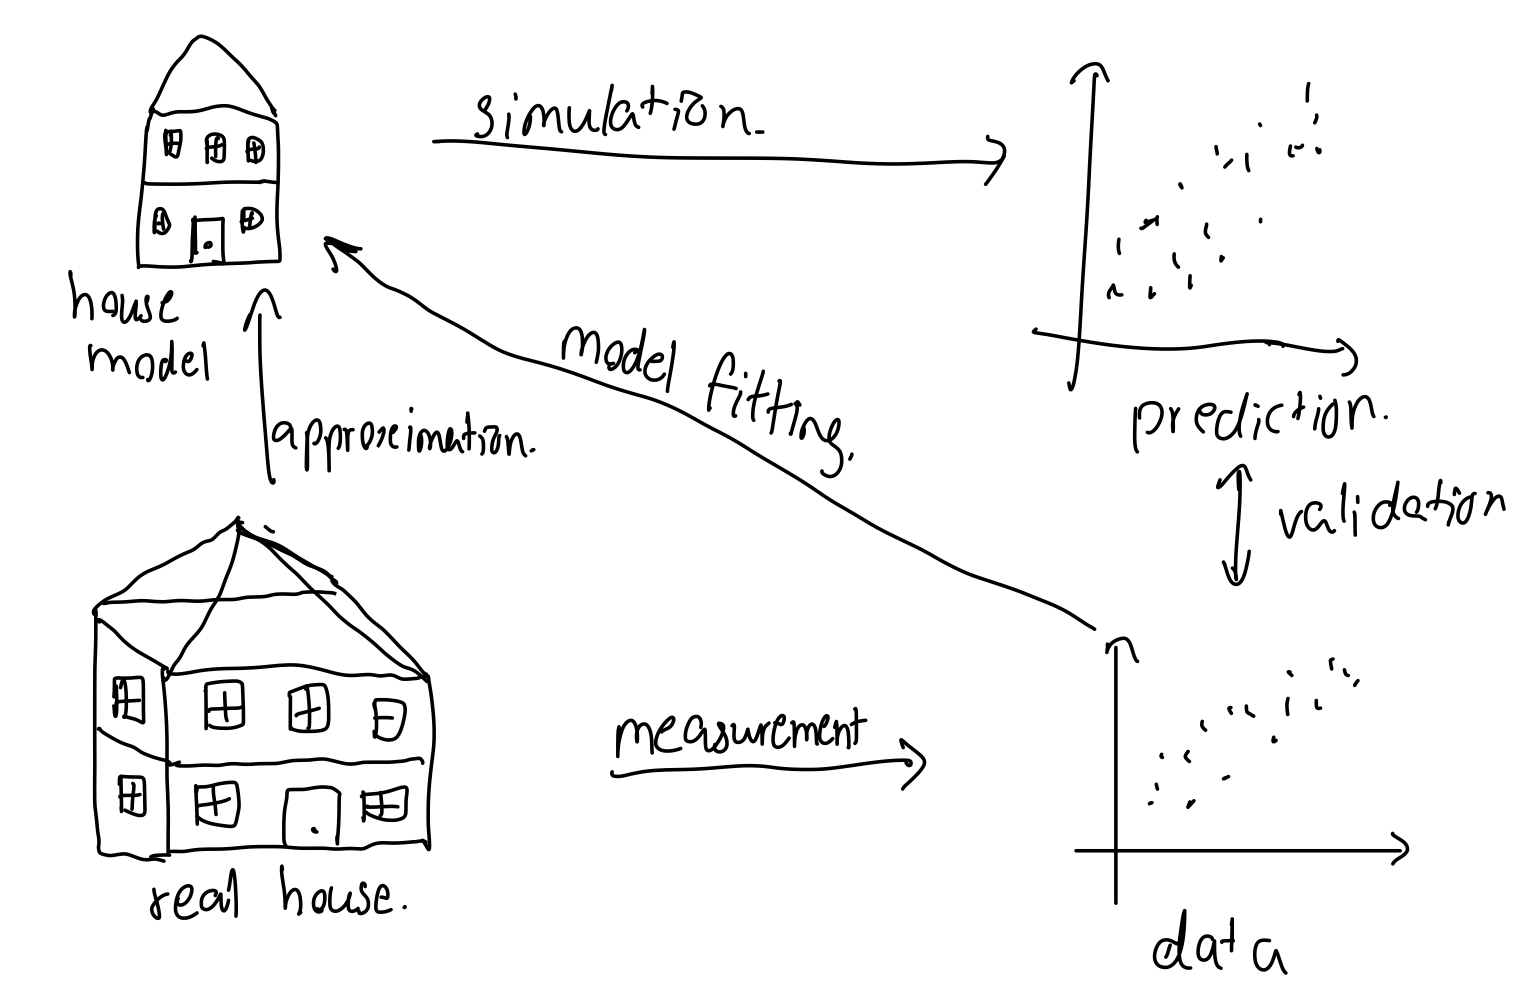
\includegraphics[width=0.75\linewidth]{IMG_88AAE0E6A79D-1.jpeg}
    \caption{Illustration of real house and house model}
    \label{fig:enter-label}
\end{figure}

\easysubproblem{Pursuant to the fix in the previous question, how do we define \emph{data} for the purposes of this class?}\spc{2}

We define data by measuring real house using metric. For example, measuring length, width and height using meters.


\easysubproblem{Pursuant to the fix in the previous question, how do we define \emph{predictions} for the purposes of this class?}\spc{3}

We define predictions by computing or simulating the model.

\easysubproblem{Why are \qu{all models wrong}? We are quoting the famous statisticians George Box and Norman Draper here.}\spc{2}

All models are wrong because we cannot perfectly capture the measurement or metric data in complex real world.

\intermediatesubproblem{Why are \qu{[some models] useful}? We are quoting the famous statisticians George Box and Norman Draper here.}\spc{2}

Some models are useful because they help to solve human's problems. For example, maps are not accurate, but they can help navigation. Weather predictions are not accurate, but they can help us what to wear the next day.

\intermediatesubproblem{What is the difference between a "good model" and a "bad model"?}\spc{2}

A good model is that when you validate the prediction or the output of the model with the real world measurement, it is close enough or accurate enough and the result is consistent. For example, F=ma is always true no matter what force, mass or acceleration. A bad model is that when you validate, it is not close enough or accurate enough and the result is inconsistent.

\end{enumerate}




\problem{We are now going to investigate the famous English aphorism \qu{an apple a day keeps the doctor away} as a model. We will use this as springboard to ask more questions about the framework of modeling we introduced in this class.}

\begin{enumerate}


\easysubproblem{Is this a mathematical model? Yes / no and why.}\spc{3}

This is not a mathematical model because it doesn't define how we can measure the doctor away. In mathematical model, there need to be an equation or it needs to define clearly what does mean by keeping the doctor away. For example, even you eat an apple a day, if you have a car accident, we are going to be hospitalized or at least, we need to see a doctor in this situation. 

\easysubproblem{What is(are) the input(s) in this model?}\spc{3}

an apple that you eat a day. It could be the size of apple, type of apple, apple with shell or not, and the time you eat an apple. 

\easysubproblem{What is(are) the output(s) in this model?}\spc{3}

The outputs in this model are how often you see a doctor in your life.\textbf{}

\intermediatesubproblem{How good / bad do you think this model is and why?}\spc{3}

This is a very bad model because it oversimplifies about not seeing a doctor with an apple. There are many other factors that can contribute to the model to judge how often a person see a doctor. We don't know what time frame we are talking about as an infant cannot eat an apple. Also, if we only use an apple, we can say this is out of sample example and the model is not accurate. 

\easysubproblem{Devise a metric for gauging the main input. Call this $x_1$ going forward.}\spc{4}

 $x_1$ = the amount of apple a person who is older than 2 years old eats per day measured in gram

\easysubproblem{Devise a metric for gauging the main output. Call this $y$ going forward.}\spc{4}

$y$ = if a person who is older than 2 years old sees a doctor either 1 is seeing a doctor and 0 is not seeing a doctor per day 

\easysubproblem{What is $\mathcal{Y}$ mathematically?}\spc{3}

Mathematically, $\mathcal{Y}$ is an output space. In this case, $\mathcal{Y}$ is {0, 1}

\easysubproblem{Briefly describe $z_1, \ldots, z_t$ in English where $y = t(z_1, \ldots, z_t)$ in this \emph{phenomenon} (not \emph{model}).}\spc{3}

$z_1, \ldots, z_t$ are true, casual input information or the true drivers of the phenomenon. In this phenomenon, $z_1, \ldots, z_t$ are the real factors that really influence if you need to see a doctor or not. For example, diet, exercise,sleep, how you wear and so on.

\easysubproblem{From this point on, you only observe $x_1$. What is the value of $p$?}\spc{1}

The value of $p$ is 1 because $p$ is the number of predictors which is $x_1$


\intermediatesubproblem{What is $\mathcal{X}$ mathematically? If your information contained in $x_1$ is non-numeric, you must coerce it to be numeric at this point.}\spc{3}

Mathematically, $\mathcal{X}$ is the set of non negative real number.

\easysubproblem{How did we term the functional relationship between $y$ and $x_1$? Is it approximate or equals?}\spc{3}

The functional relationship between $y$ and $x_1$ is approximation. It is impossible to get the perfect function for $x_1$ to generate $y$ as we cannot solve f analytically. Moreover, there are always errors due to ignorance.

\easysubproblem{Briefly describe \emph{superivised learning}.}\spc{5}

Learning is that we are collecting the information or data from varieties of sources. Experience is also a kind of learning. Supervised means someone is guiding or learning from the historical data or information. So, supervised learning means that a model is learning from the historical data including input and output and you are supervising these learning algorithm based on previous examples that occured.

\easysubproblem{Why is \emph{superivised learning} an \emph{empirical solution} and not an \emph{analytic solution}?}\spc{3}

Supervised learning is an empirical solution and not an analytic solution because it is learning from historical data and it cannot be learn or solve using mathematical methods such as using calculus or other operations to solve the problem.

\intermediatesubproblem{From this point on, assume we are involved in supervised learning to achieve the goal you stated in the previous question. Briefly describe what $\mathbb{D}$ would look like here.}\spc{3}

$\mathbb{D}$ would look like a historical data set of inputs which are the data of grams of apple that a person eats a day and the outputs which are the data of if a person goes to see a doctor or not. 

\intermediatesubproblem{Briefly describe the role of $\mathcal{H}$ and $\mathcal{A}$ here.}\spc{3}

$\mathcal{H}$ represents the hypothesis space, the set of candidate functions that approximate the true relationship between apple consumption and the likelihood of seeing a doctor. $\mathcal{A}$ is the learning algorithm that, given the data $\mathbb{D}$, selects the best function $ g \in \mathcal{H} $ that best predicts whether a person needs to see a doctor based on their apple consumption.


\easysubproblem{If $g = \mathcal{A}(\mathbb{D}, \mathcal{H})$, what should the domain and range of $g$ be?}\spc{3}

The domain of  $g$  is  $X = \mathbb{R}_{\geq 0}$ , the set of non-negative real numbers for the amount of apple in gram and the range of $g$ is {0, 1} which 0 means a person doesn't see a doctor and 1 means a person see a doctor.

\easysubproblem{Is $g \in \mathcal{H}$? Why or why not?}\spc{3}

Yes,  $g \in \mathcal{H}$  because  $g$ is a specific function chosen from the hypothesis space $\mathcal{H}$ by the learning algorithm $\mathcal{A}$.

\easysubproblem{Given a never-before-seen value of $x_1$ which we denote $x^*$, what formula would we use to predict the corresponding value of the output? Denote this prediction $\hat{y}^*$.}\spc{1}


$\hat{y}^* = g(x^*)$ where $\hat{y}^*$ is future prediction, $x^*$ is the future observation  and $g$ is the best function to compute the future prediction


\intermediatesubproblem{$f$ is the function that is the best possible fit of the phenomenon given the covariates. We will unfortunately not be able to define \qu{best} until later in the course. But you can think of it as a device that extracts all possible information from the covariates and whatever is left over $\delta$ is due exclusively to information you do not have. Is it reasonable to assume $f \in \mathcal{H}$? Why or why not?}\spc{2}

It is not reasonable to assume $f \in \mathcal{H}$ because $f$ represents the true, often highly complex real-world function, while $\mathcal{H}$ is a limited set of approximations. 


\easysubproblem{In the general modeling setup, if $f \notin \mathcal{H}$, what are the three sources of error? Copy the equation from the class notes. Denote the names of each error and provide a sentence explanation of each. Denote also $e$ and $\mathcal{E}$ using underbraces / overbraces.}\spc{6}

\[
y = g(\vec{x}) + h^*(\vec{x}) - g(\vec{x}) + f(\vec{x}) - h^*(\vec{x}) + t(\vec{x}) - f(\vec{x})
\]
\[
y = g(\vec{x}) 
    + h^*(\vec{x}) - g(\vec{x})
    + f(\vec{x}) - h^*(\vec{x})
    + \underbrace{t(\vec{x}) - f(\vec{x})}_{{\sigma}}
\]

\[
y = g(\vec{x}) 
    + h^*(\vec{x}) - g(\vec{x})
    + \underbrace{f(\vec{x}) - h^*(\vec{x})
    + t(\vec{x}) - f(\vec{x})}_{\mathcal{E}}
\]

\[
y = g(\vec{x}) 
    + \underbrace{h^*(\vec{x}) - g(\vec{x})
    + f(\vec{x}) - h^*(\vec{x})
    + t(\vec{x}) - f(\vec{x})}_{{e}}
\]

The three sources of error are ignorance error which is ($t-f$), misspecification error which is ($f-h^*$) and estimation error which is ($h^* - g$). Ignorance error is an error that arises from factors that are entirely unknown or unobservable in our dataset. Misspecification error occurs when the best possible function within our hypothesis space $(\mathcal{H})$ does not perfectly match the true function  f.  Estimation error arises due to limitations in learning the best function  $h^*$  from finite data. 


\easysubproblem{In the general modeling setup, for each of the three source of error, explain what you would do to reduce the source of error as best as you can.}\spc{7}

We can increase $x$ to reduce ignorance error. We can choose more expansive $(\mathcal{H})$ to be more complicated and more expressive of complex relationships to reduce the misspecification error. We can improve $(\mathcal{A})$ by increasing sample size $n$  to decrease the estimation error.

\intermediatesubproblem{In the general modeling setup, make up an $f$, an $h^*$ and a $g$ and plot them on a graph of $y$ vs $x$ (assume $p=1$). Indicate the sources of error on this plot (see last question). Which source of error is missing from the picture? Why?}\spc{9}

\begin{figure}[h]
    \centering
    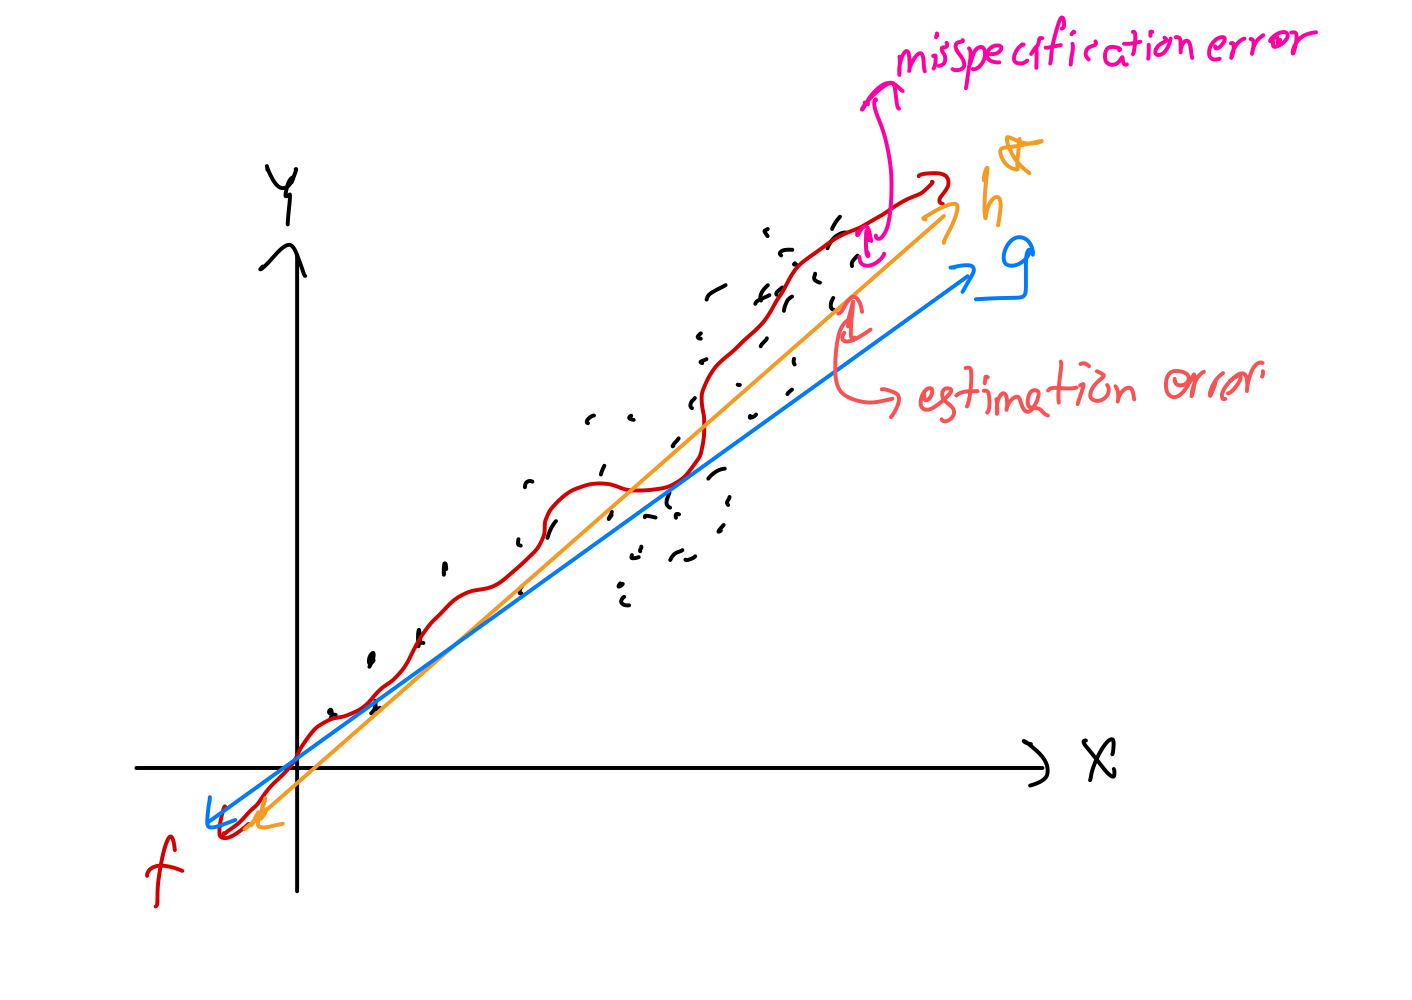
\includegraphics[width=0.75\linewidth]{IMG_2A47C0BC95B4-1.jpeg}
    \caption{general modeling setup}
    \label{fig:enter-label}
\end{figure}

Ignorance error is missing from the picture because we can never truly know the underlying function  $t$ , which represents the true causal mechanism behind the data. Instead, we approximate with  $f$ , which introduces inherent limitations in any model.

\easysubproblem{What is a null model $g_0$? What data does it make use of? What data does it not make use of?}\spc{3}

A null model $g_0$ is the model that we use if we did not have any $x$ or anything about the units except the actual final response. We could also say $g_0$ is a dummy or bad model like a default one. It makes use of the data the are from $\mathbb{D}$ which is equal to $\vec{y}$ and it doesn't make use of any data or feature that influences the function.


\easysubproblem{What is a parameter in $\mathcal{H}$?}\spc{3}

$\mathbb{H} = \{ \mathbb{1}_{x \ge \theta} \mid \theta \in \mathbb{R} \}$ 

A parameter in $\mathcal{H}$ is $\theta$ which belongs to  $\mathbb{R}$ . This threshold  $\theta$ controls the point at which the function transitions from 0 to 1. In our example, we could say $\theta$ is 150 gram of apple a day or a certain value.

\easysubproblem{Regardless of your answer to what $\mathcal{Y}$ was above in (g), we now coerce $\mathcal{Y} = \braces{0,1}$. What would the null model $g_0$ be and why?}\spc{2}

The null model $g_0$ would be Mode$[\vec{y}]$ which mean whatever(0 or 1) appears most in $y$ will be $g_0$.

\easysubproblem{Regardless of your answer to what $\mathcal{Y}$ was above in (g), we now coerce $\mathcal{Y} = \braces{0,1}$. If we use a threshold model, what would $\mathcal{H}$ be? What would the parameter(s) be?}\spc{2}

$\mathbb{H} = \{ \mathbb{1}_{x \ge \theta} \mid \theta \in \mathbb{R} \}$ where the hypothesis space  $\mathcal{H}$  consists of all indicator functions that can predict if a person needs to seed a doctor where the prediction is determined by whether the input $x$ which is the amount of apple that a person eats exceeds a certain threshold  $\theta$ .

\easysubproblem{Give an explicit example of $g$ under the threshold model.}\spc{1}

$\mathbb{H} = \{ \mathbb{1}_{x \ge 100} \}$ where x is the daily amount of apple consumption in grams and $\theta = 100$

This means that if a person eats 100g or more on a day, he will not see a doctor on that day.

\end{enumerate}


\problem{As alluded to in class, modeling is synonymous with the entire enterprise of science. 

In 1964, \href{https://en.wikipedia.org/wiki/Richard_Feynman}{Richard Feynman}, a famous physicist and public intellectual with an inimitably captivating presentation style, gave a series of seven lectures in 1964 at Cornell University on the \qu{character of physical law}. Here is a \href{https://www.youtube.com/watch?v=EYPapE-3FRw}{10min excerpt} of one of these lectures about the scientific method. Feel free to watch the entire clip, but for the purposes of this class, we are only interested in the following segments: 0:00-1:00 and 3:48-6:45. }

\begin{enumerate}


\intermediatesubproblem{According to Feynman, how does the scientific method differ from learning from data with regards to building models for reality? (0:08)}\spc{3}

The scientific method differs from learning from data with regards to building models for reality by guessing the law first. When learning from data, we need to measure numerically first. Then create a model. Then, simulate or compute the model to validate with the reality. In scientific method, we compute the sequences of the guess to see the law that we guessed is right and compare the computation with the nature. If it disagrees with the experiment, the guessed law is wrong no matter what the guess or no matter the person is smart. 

\intermediatesubproblem{He uses the phrase \qu{compute consequences}. What word did we use in class for \qu{compute consequences}? This word also appears in your diagram in 2a. (0:14)}\spc{1}

Simulation/ Computation. 


\intermediatesubproblem{When he says compare consequences to \qu{experiment}, what word did we use in class for \qu{experiment}? This word also appears in your diagram in 2a. (0:29)}\spc{1}

data. Data that we measure from the reality.

\intermediatesubproblem{When he says \qu{compare consequences to experiment}, which part of the diagram in 2a is that comparison?}\spc{1}

Validation Part 

\hardsubproblem{When he says \qu{if it disagrees with experiment, it's wrong} (0:44), would a data scientist agree/disagree? What would the data scientist further comment?}\spc{3}

A data scientist would agree to what he says. The data scientist would try other methods for the experiment such as trying with more data or trying different algorithm. He would see if the experiment is close enough or the error is minimized, he could use the model to get an approximate answer.

\hardsubproblem{[You can skip his UFO discussion as it belongs in a class on statistical inference on the topic of $H_0$ vs $H_a$ which is \emph{not} in the curriculum of this class.] He then goes on to say \qu{We can disprove any definite theory. We never prove [a theory] right... We can only be sure we're wrong} (3:48 - 5:08). What does this mean about models in the context of our class?}\spc{3}

We can disprove any model by checking the measurement we get from reality. However, we cannot prove if a model is right. The reason is the the data we get from real world could be change in the future or the amount of the data could also change the result of the model. That's why we can only be sure we are wrong and cannot say the model is completely right.

\hardsubproblem{Further he says, \qu{you cannot prove a \emph{vague} theory wrong} (5:10 - 5:48). What does this mean in the context of mathematical models and metrics?} \spc{3}

In the context of mathematical models and metrics, since it is vague, we do not have any information, variables or features or the interpretation could be misleading to falsify the model. Moreover, mathematical models need to have clear assumptions and specific variable so that we can clearly define what to or how to falsify the model. Similarly, in metrics, unclear evaluation criteria can lead to misleading conclusions.


\hardsubproblem{He then he continues with an example from psychology. Remeber in the 1960's psychoanalysis was very popular. What is his remedy for being able to prove the vague psychology theory right (5:49 - 6:29)?} \spc{2}

His remedy for being able to prove the vague psychology theory right is the looking ahead of time and measure what limit or threshold is correct or incorrect. By using his example, if we want to find out why her child hates her because she didn't caress him or love him enough when he was a child, we need to know the numerical measurement of how much love exactly is not enough and how much love exactly is overindulgent.

\hardsubproblem{He then says \qu{then you can't claim to know anything about it} (6:40). Why can't you know anything about it?} \spc{3}

We can't know anything about it because we are dealing with psychological matters that things cannot be defined so precisely.

\vspace{1cm}

Just to demonstrate that this modeling enterprise is all over science (not just Physics), I present to you the controversial theoretical political scientist John Mearsheimer. He's all over youtube and there's nothing special about this video that I will link here about \href{https://www.youtube.com/watch?v=D_Mx_e8t7nU&t=4673s}{Can China Rise Peacefully?} Feel free to watch the entire clip, but for the purposes of this class, we are only interested in the following segments referenced in the questions which has nothing to do with China, only his theory of \qu{power politics}.

\hardsubproblem{Is Mearsheimer's model of great power politics / international relations (i.e., modern history) 9:35-17:22 simple or complicated? Explain.} \spc{3}

Mearsheimer’s model is simple on the surface because its five assumptions are intuitive and easy to grasp and those 5 assumptions can give you general overview of power. However, when analyzed deeply, it becomes complex due to the challenge of predicting state intentions—since intentions exist in leaders’ minds and are inherently uncertain. Moreover, there are other factors that might influence the power of a contry.



\hardsubproblem{Summarize his ideas about limitations of his theory from 39:18-40:00 using vocabulary from this class.} \spc{3}

To summarize, Theory are essential and we should not be condemnation of theory, even the theory is 25\% of the time wrong which is 75\% of the time is correct. We need to understand the limitation of the theory as some important factors could left out. However, theory simplifies a complicated reality. Speaking in the context of our class, we are using some factors from the complex reality to build a model(theory) that can predict the phenomenon. We need to aware that our model is always wrong as we might left to add some factors/ features that is essential for the model. However, although all the model are wrong, some are useful and we are trying to make a model which is wrong but we will make less error so that it is useful in someplace.


\end{enumerate}

\end{document}

\end{document}

%%%%%%%%%%%%%%%%%This following will go in the next homework!!!



\problem{These are questions about the linear perceptron. This problem is not related to problem 3.}

\begin{enumerate}

\easysubproblem{For the linear perceptron model and the linear support vector machine model, what is $\mathcal{H}$? Use $b$ as the bias term.}\spc{3}

\intermediatesubproblem{Rewrite the steps of the \emph{perceptron learning algorithm} using $b$ as the bias term.}\spc{13}

\easysubproblem{Illustrate the perceptron as a one-layer neural network with the Heaviside / binary step / indicator function activation function.}\spc{10}

\easysubproblem{Provide an illustration of a two-layer neural network. Be careful to indicate all pieces. If a mathematical object has a different value from another mathematical object, denote it differently.}\spc{10}

\end{enumerate}